%!TEX root = index.tex
\chapter{Data}

This chapter summarizes which data were used for implementation and testing of the module for air traffic control simulation in terminal area. The design and implementation of the module is general and can be used for simulation of any TMA sector but in order to test its functionality concrete sector description and air traffic scenario must be used. It was important to have all the data relevant to the test sector available because any of them missing would cause the whole scenario to be unusable.

\section{Hartsfield–Jackson Atlanta International Airport}

\begin{figure}[h]
    \centering
    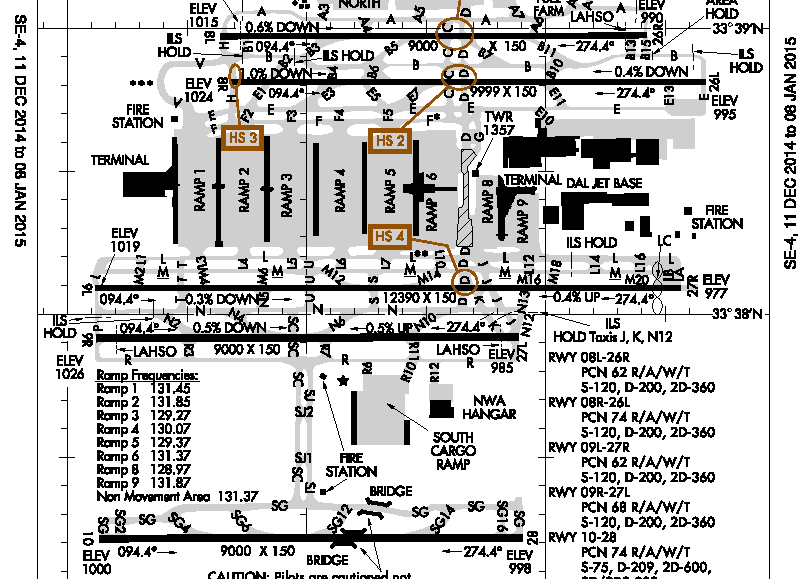
\includegraphics[width=0.8\textwidth]{figures/atlanta-diagram.pdf}
    \caption{Section of the airport diagram of the Hartsfield–Jackson Atlanta International Airport \cite{atlanta-diagram}}
    \label{fig:atlanta-diagram}
\end{figure}

Hartsfield–Jackson Atlanta International Airport (ICAO code KATL) has been the world's busiest airport by passenger traffic since 1998 with more than 94 million passengers in 2013. It has also the most landings and take-offs since 2005. The airport has 207 domestic and international gates which is the most at any airport. \cite{atlanta}

This airport was chosen because the amount of traffic would provide more interesting test-case in comparison to some other, less busy airport. Also all the other required data were available for Atlanta Airport.

The goal of this thesis is to simulate the approach phase of the flight, from the moment airplane leaves en-route sector to touchdown on the runway. The ground movement is not simulated and therefore the only information needed about the airport is the configuration of its runways.

The runway configuration is publicly available on the FAA website \cite{atlanta-diagram}. Airport runway configuration including positions and elevations of each runway was created in a form of XML file that can be used in AgentFly simulation.

The Atlanta Airport has five runways, the southernmost (\texttt{10/28}) is used for cargo aircraft and was therefore eliminated from the scenario. Out of the four remaining runways the inner two (\texttt{8R/26L} and \texttt{9L/27R}) are used exclusively for departures and only the outer two runways (\texttt{8L/26R} and \texttt{9R/27L}) are used for incoming flights. These two runways will be used in the test simulation scenarios. Figure \ref{fig:routes} shows all the Atlanta Airport runways (in yellow) as they are shown in AgentFly visualization.

\section{Atlanta TMA}

Together with the description of the Atlanta Airport itself, the definition of surrounding TMA sector was needed. This sector describes the area of authority of approach control service. The name of the TMA sector is \texttt{A80}. As the Atlanta Airport is one of the busiest airports, the associated TMA sector is defined as Class B airspace. The definition of the airspace is provided by Federal Aviation Administration \cite{atlanta-tma}.

\begin{figure}[H]
    \centering
    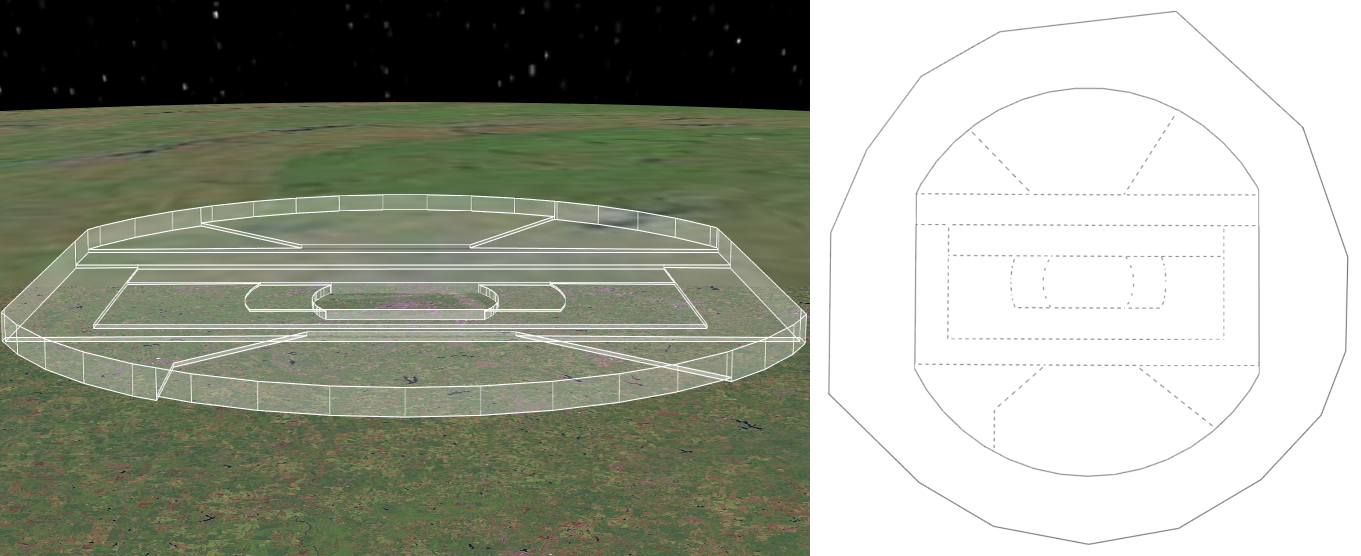
\includegraphics[width=\textwidth]{figures/tracon.png}
    \caption{Left: Atlanta Class B airspace in AgentFly 3D visualization, Right: The airspace as shown on radar screen in AgentFly with borders of neighboring en-route sectors}
    \label{fig:tracon}
\end{figure}

The definition of the airspace isn't available in a computerized form ready for machine processing and had to be converted to XML sector definition by hand from the available textual description \cite{atlanta-tma}. The resulting sector as seen in agentFly visualization is shown in Figure \ref{fig:tracon}. Problem with this TMA definition is that there is a gap between TMA border border and previously provided neighboring en-route sectors making it impossible to hand-off planes from one sector to the other. Upon consulting with FAA, for the purposes of testing the borders of surrounding en-route sectors were used for TMA definition  instead of the Class B airspace itself. This way the TMA sector touches the en-route sectors allowing airplane hand-offs. The comparison between Class B airspace and used sector definition is shown in Figure \ref{fig:tracon} right. The TMA sector and some neighboring en-route sectors is also shown in Figure \ref{fig:routes} left, note that the sectors do not overlap, the en-route sectors horizontally touch the TMA sector and partly extend above it.

\section{STARs}

STARs are routes that connect the en-route sectors and lead the airplanes to the runways. They define the path itself as well as safe intervals for altitude and speed for selected fixes on the route. The routes are designed in such way that if they cross horizontally, the separation is ensured vertically. This means that once a plane is flying on a STAR route there is no risk of collision with aircraft flying on other routes.

\begin{figure}[h]
    \centering
    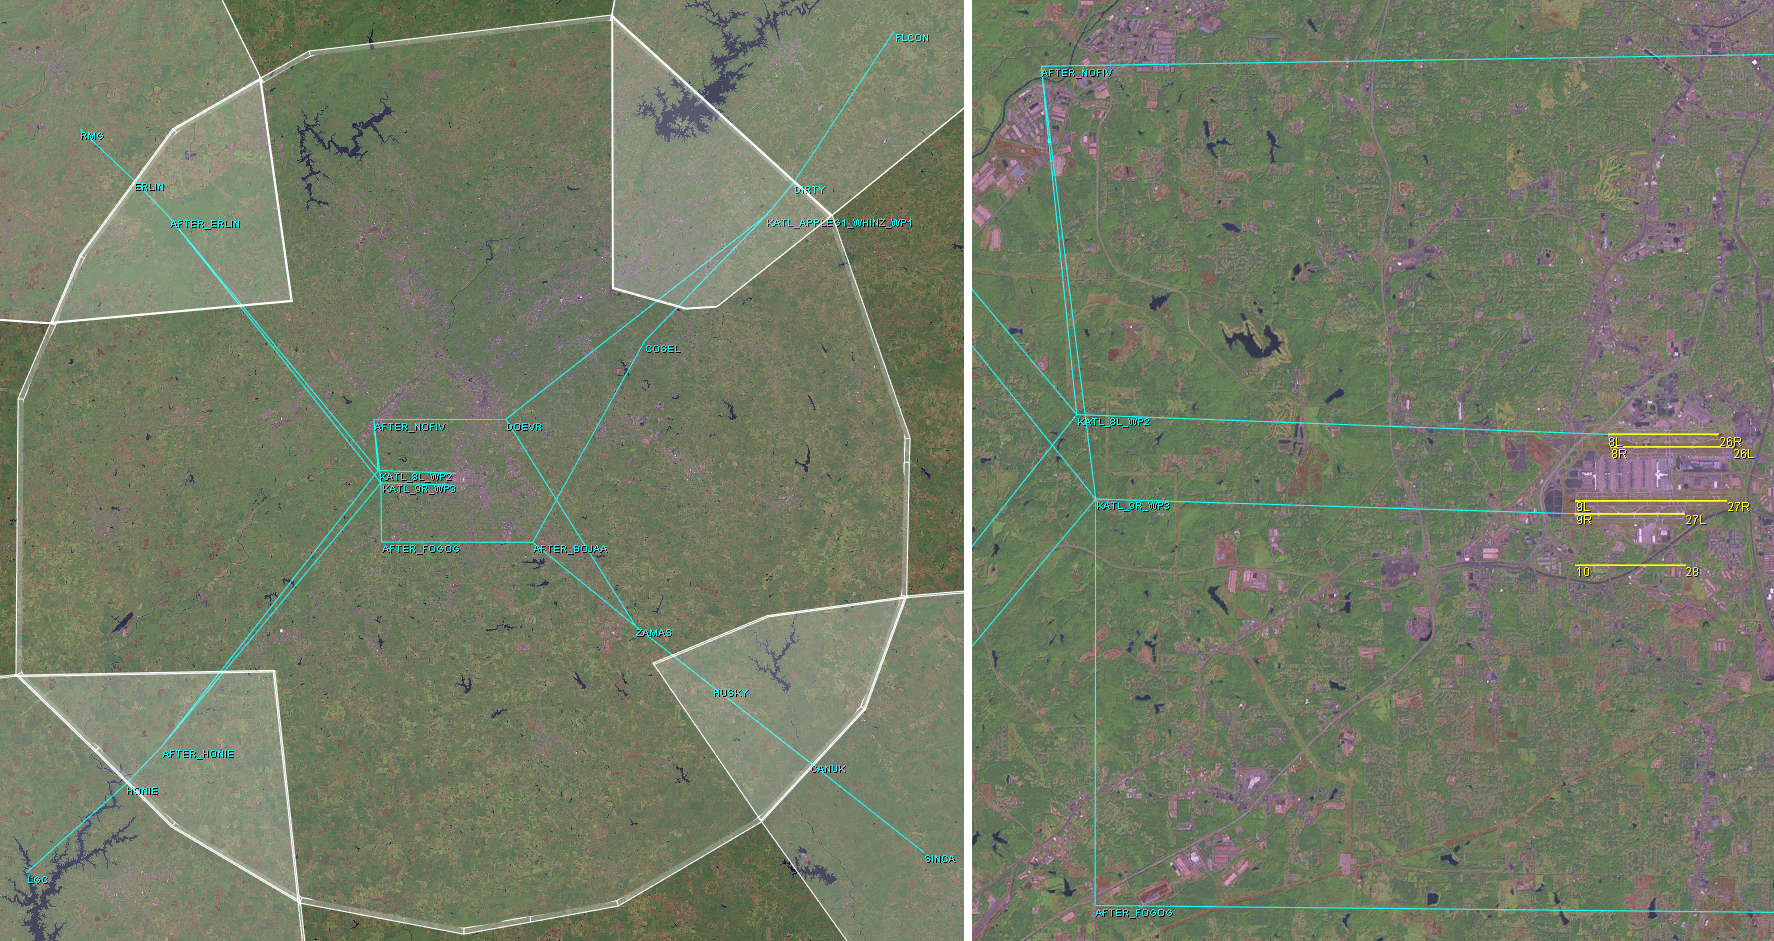
\includegraphics[width=\textwidth]{figures/routes.png}
    \caption{STARs near Atlanta Airport, Right: overall view, Left: detailed view of the configuration near runways}
    \label{fig:routes}
\end{figure}

The STAR definitions are made publicly available by the FAA in non-machine readable format but were also provided for the purpose of TMA simulation in AgentFly in computerized proprietary format. The provided STAR descriptions were used in this thesis even though they do not correspond entirely with the publicly provided data. SID routes were also provided but not used as simulation of takeoff was not part of the thesis.

Figure \ref{fig:routes} shows the loaded routes for eastern operation of Atlanta Airport in AgentFly visualization. Atlanta Airport can function in two configurations depending on the prevailing wind direction. The approaches and take-offs can be performed either in western or eastern direction. The route configuration is basically identical, only mirrored along the north-south axis. AgentFly doesn't simulate the wind at the moment and therefore static eastern direction was used for the testing purposes.

\section{Flights}

Recording of real-world 24 hour traffic in Atlanta Air Route Traffic Control Center (ZTL) on 20th June 2013 was provided by FAA for testing. The log files contain records of 7832 flights. Out of those VFR flights were filtered out because only IFR flights are simulated in AgentFly. Also aircraft of unusual type that can not be simulated using BADA simulation models were removed from the test data. Also flights flying through the \texttt{A80} sector or taking of at the Atlanta Airport were filtered from the logs leaving 1308 flights arriving to the airport.

\begin{figure}[h]
    \centering
    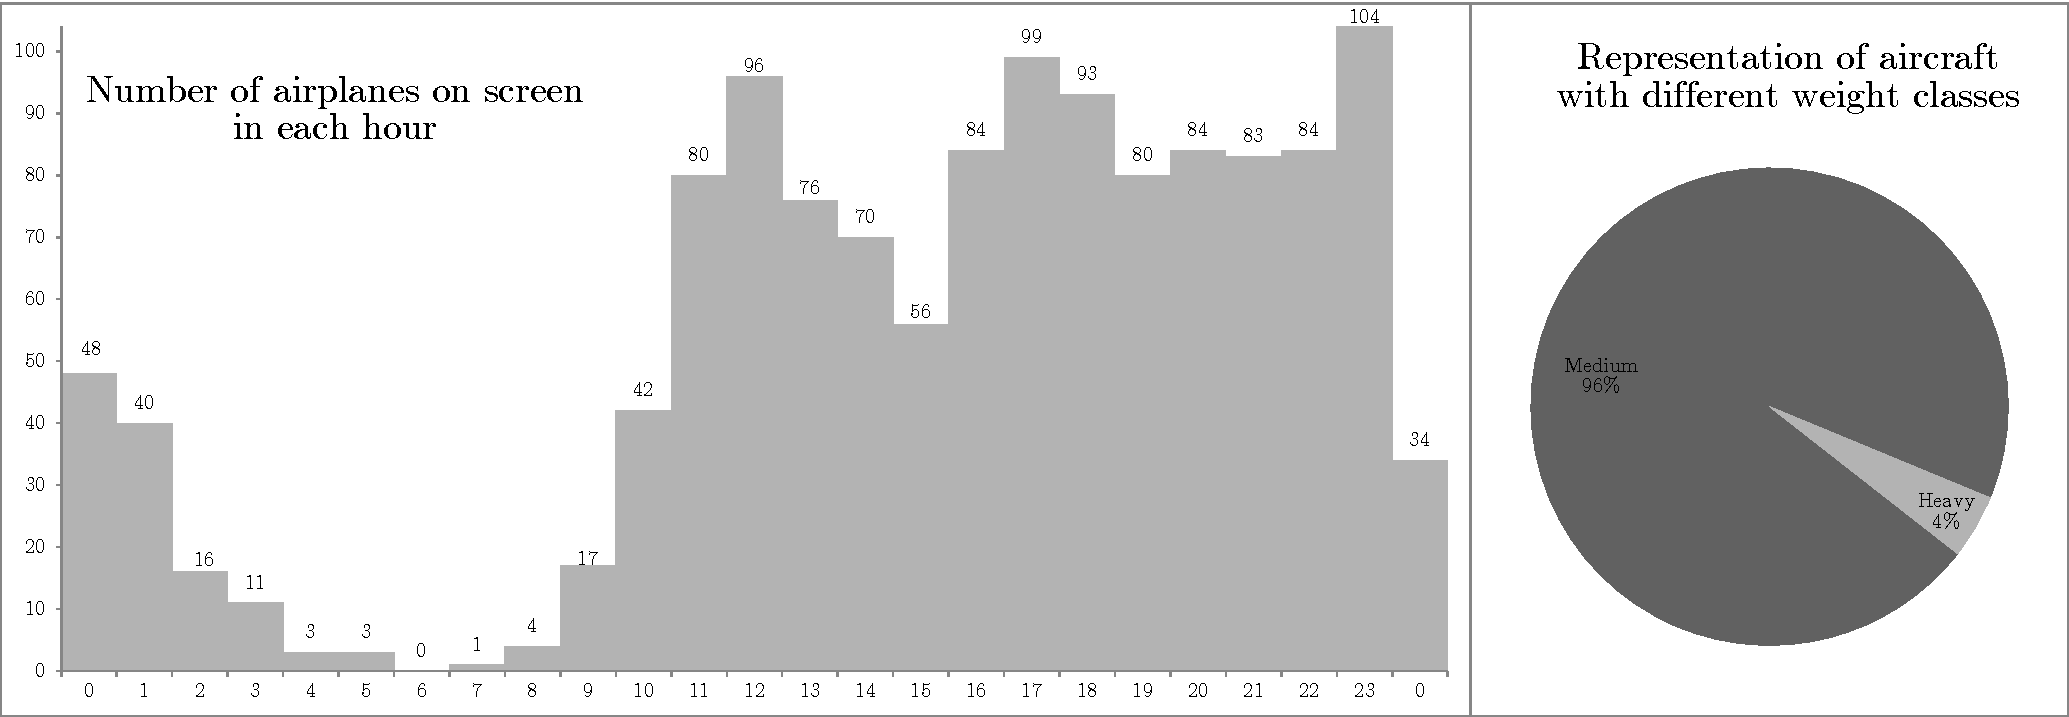
\includegraphics[width=\textwidth]{graphs/real-flights.pdf}
    \caption{Left: histogram of number of airplanes appearing on screen in each hour of the simulated 24 hours traffic, Right: graph of representation of aircraft with different weight classes in the test air traffic}
    \label{graph:flights}
\end{figure}

Figure \ref{graph:flights} shows the histogram of number of airplanes appearing on screen in each hour and graph of representation of aircraft with different weight classes in the air traffic. The histogram demonstrates the usual progress of the traffic during the day with decline in early morning and peaks around noon and in the evening. The pie chart shows that the traffic going to the Atlanta Airport is rather monotonous 96\% of medium weight aircraft, 4\% heavy aircraft and no light or super heavy planes. Therefore additional test scenario was created to test the scheduling algorithms in situations with more variable composition of arriving flights.